\label{sec:empirical}

\begin{figure}[t!]
\center
\includegraphics[width=0.48\textwidth]{Figures/rover1D/roverLinear1d2V6.pdf} 
\vspace{-3mm}
\caption{\footnotesize Value function at iteration 6 for $\MarsRoverUni$, showing how different levels of approximation error (eps) lead to different compressions.}
\label{fig:rover1dv6} 
\vspace{-3mm}
\end{figure}

In this section we wish to compare the scalability of exact SDP
(calling BASDP in Algorithm~\ref{sec:basdp} with $\epsilon=0$)
vs. various levels of approximation error $\epsilon > 0$ to determine
the trade-offs between time and space vs. approximation error.
To do this, we evaluated BASDP on three different domains ---
\MarsRoverUni, \MarsRoverBi and \Invent --- detailed next.

\MarsRoverUni:
A unidimensional continuous Mars Rover domain motivated by
Bresina {\it et al}~\cite{bresina02} used in order to visualize the
value function and the effects of varying levels of approximation.
The position of the rover is represented by a single continuous
variable $x$ and the goal of the rover is to take pictures at
specific positions.  There is only one action $\mathit{move}(a_x)$,
where $a_x$ is the movement distance. In the description of the
problem for the instance shown below, there are two picture
points and taking pictures is recorded in two boolean variables
($tp_1$ and $tp_2$). The dynamics for deterministic action $move(a_x)$ are as
follows: {\footnotesize
\vspace{-2mm}
\begin{align*}
tp_1' &= \begin{cases}
tp_1 \vee (x>40 \wedge x<60)&: 1.0\\
else&: 0.0\\
\end{cases}\\
tp_2' &= \begin{cases}
tp_2 \vee (x>-60 \wedge x<-40)&: 1.0\\
else&: 0.0\\
\end{cases}\\
x' &=  x +a_x\\
R & = R_1 + R_2 - 0.1*|a_x|\\
%R & = R_1 + R_2 + R_3\\
R_1 & = \begin{cases} 
(tp_1') \wedge (\neg tp_1) \wedge (x > 50) &: 40 - 0.2*(x -50)\\
(tp_1') \wedge (\neg tp_1) \wedge (x < 50) &: 40 - 0.2*(50-x)\\
(tp_1') \wedge ( tp_1) &:  1.1\\
else &: -2\\
\end{cases} \\
R_2 & = \begin{cases} 
(tp_2') \wedge (\neg tp_2) \wedge (x > -50) &: 60 - 0.2*(-x +50)\\
(tp_2') \wedge (\neg tp_2) \wedge (x < -50) &: 60 - 0.2*(x +50)\\
(tp_2') \wedge ( tp_2) &:  1.2\\
else &: -1\\
\end{cases} \\
%R_3 & = \begin{cases} 
%a_x > 0 &: -0.1*a_x\\
%a_x < 0 &: 0.1*a_x\\
%\end{cases} \\
\end{align*} }
\vspace{-12 mm}

In Figure~\ref{fig:rover1dv6}, we plot different value functions obtained by compressing with different levels --- we note that in general larger $\epsilon$ results in a looser fit, but there are exceptions, owing to the greedy nature of successive pairwise merging for XADDs described in Section~\ref{sec:approx}.

\MarsRoverBi: In this multivariate version of a \MarsRover~domain %there are no picture points but
 the rover is expected to follow a path. The position is represented by a pair of continuous variables $(x,y)$. There is only one action, $move(a_x,a_y)$, where $|a_x| < 10$ and $|a_y| < 10$. The new position is given by $(x',y') = ( x+a_x, y+a_y)$. The reward increases with $x$ and decreases with the absolute value of $y$, that is:

\vspace{-6mm}
{\footnotesize
\begin{align*}
R & = \begin{cases}
(x \!>\! y +25) \wedge (x \!>\! - y  +25) \wedge (y \!>\!0): &\!\!-10 + x -y\\
(x \!>\! y +25) \wedge (x \!>\! - y  +25) \wedge (y \!<\!0): &\!\!-10 + x +y\\
else: & -1\\
\end{cases}
\end{align*}}
\vspace{-6mm}

\begin{figure*}[p!]
\centering
\subfigure[Value at $6^{th}$ iteration for exact SDP.] {
	 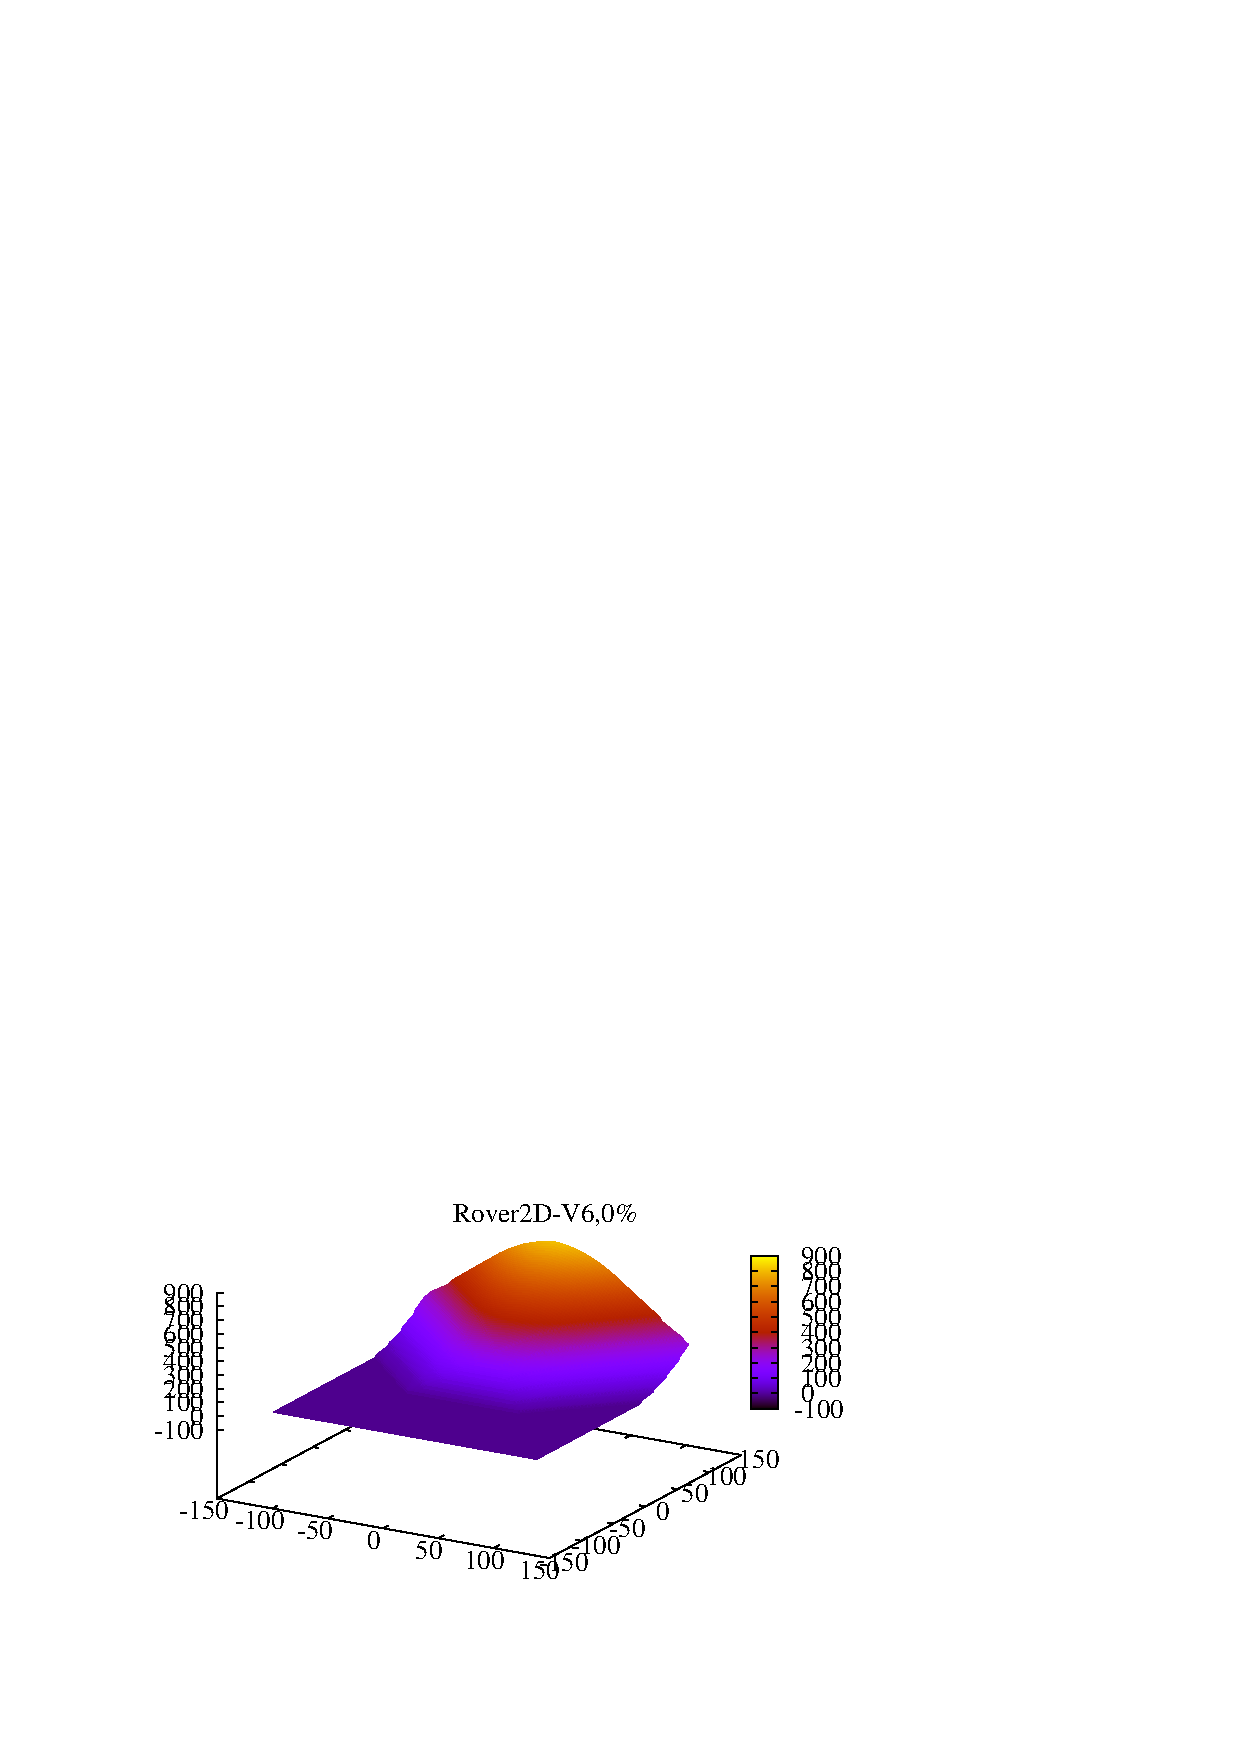
\includegraphics[width=0.45\textwidth, height=0.3\textwidth]{Figures/rover2D/rover2dV6-0.pdf}
	 \includegraphics[width=0.45\textwidth, height=0.3\textwidth]{Figures/rover2D/rover2dV6-0xadd.pdf}
	 \label{V6-0xadd}
}
\subfigure[Value at $6^{th}$ iteration for $5\%$ approximate SDP.] {
	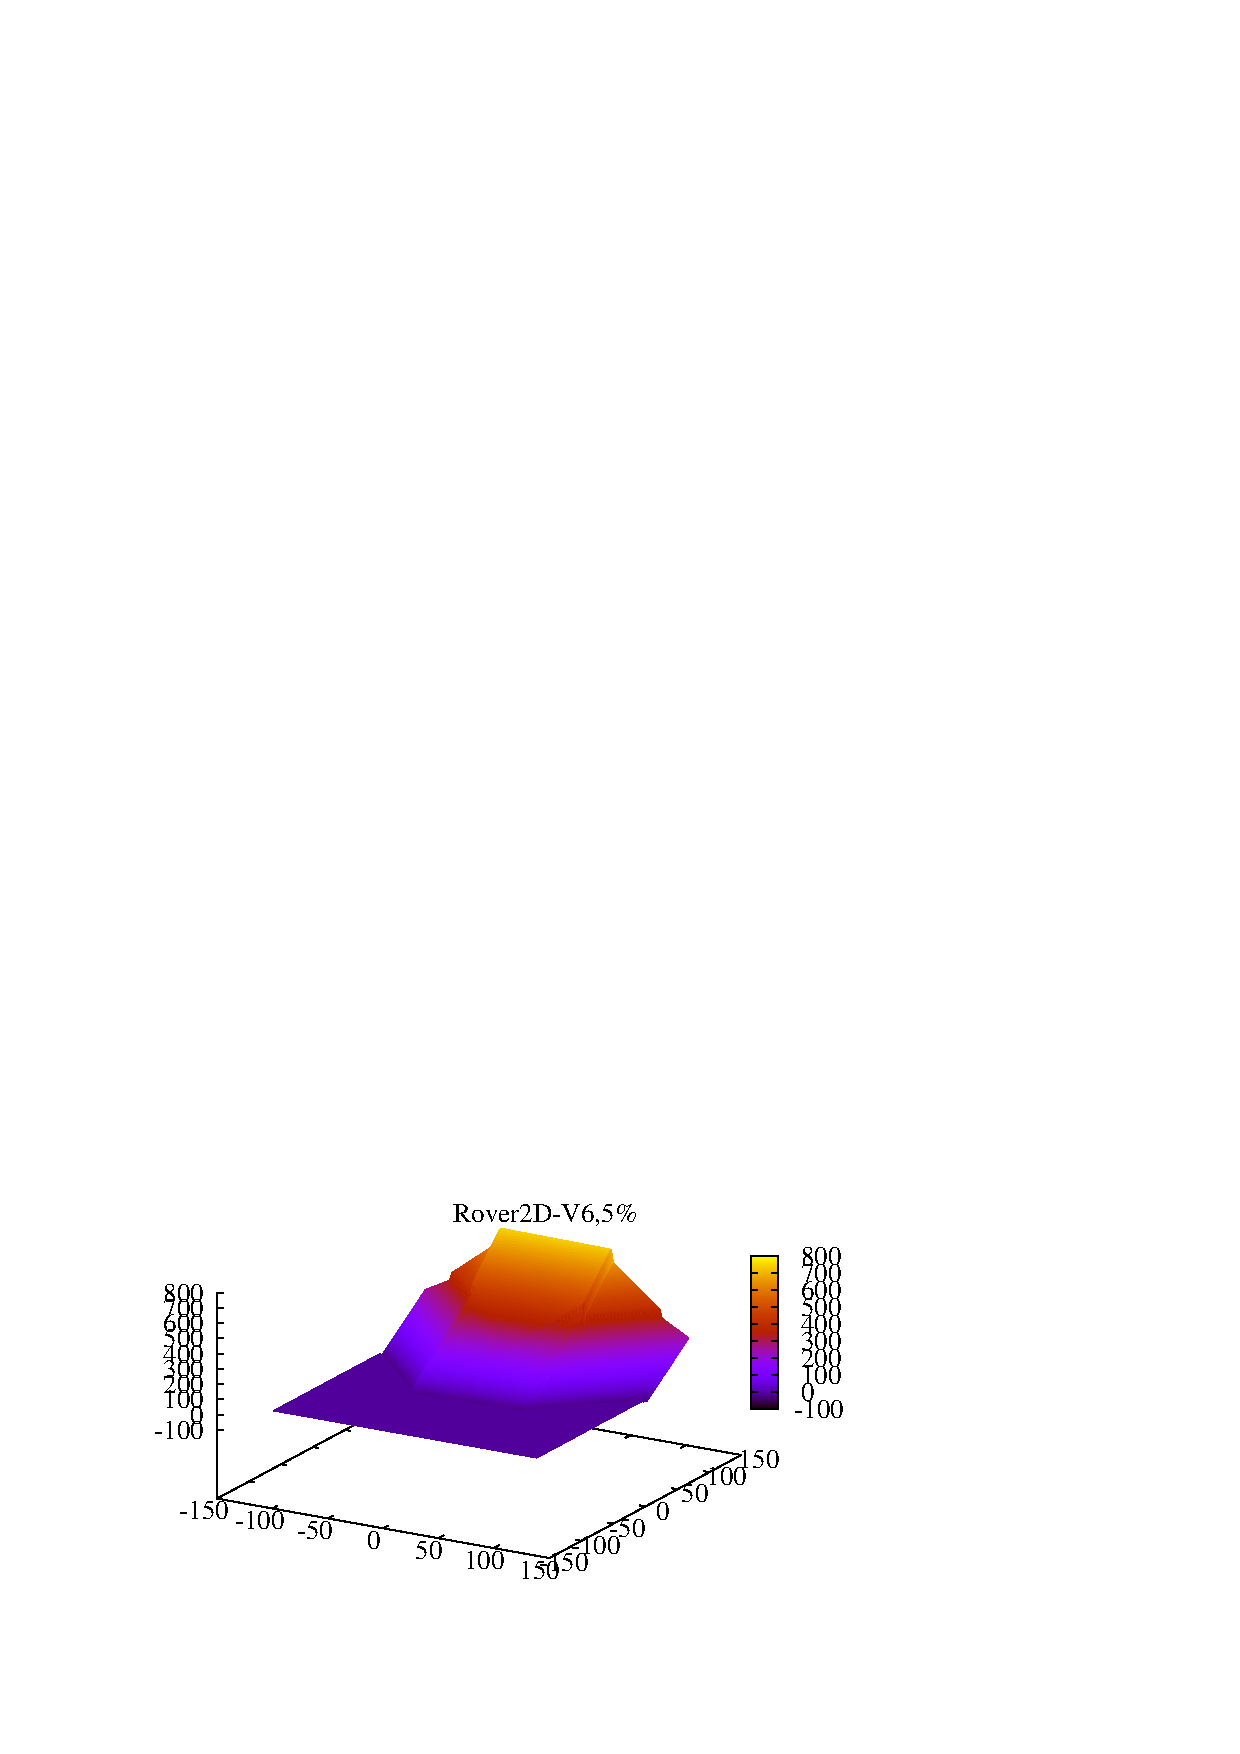
\includegraphics[width=0.45\textwidth, height=0.3\textwidth]{Figures/rover2D/rover2dV6-5.pdf}
	\includegraphics[width=0.45\textwidth, height=0.3\textwidth]{Figures/rover2D/rover2dV6-5xadd.pdf}
	 \label{V6-5xadd}
}
\caption {\footnotesize
	Value function at iteration 6 for the \MarsRoverBi domain;
	{\it (a)} Exact value function; 	{\it (b)} Approximate value function with error bounded 5\% per iteration;
	{\it (left)} 3D Plots; {\it (right)} XADD Diagrams.
}
\label{fig:Mars2DV6}
\vspace{-5mm}
\end{figure*}

\begin{figure*}[tbph!]
\centering
\includegraphics[width=0.32\textwidth]{Figures/inventory/inventory2Nodes.pdf}
\hspace{1mm}
\includegraphics[width=0.32\textwidth]{Figures/inventory/inventory2Time.pdf}
\hspace{1mm}
\includegraphics[width=0.32\textwidth]{Figures/inventory/inventory2MaxErr.pdf}
\\
\vspace{5mm}
\includegraphics[width=0.32\textwidth]{Figures/rover2D/rover2d-Nodes.pdf}
\hspace{1mm}
\includegraphics[width=0.32\textwidth]{Figures/rover2D/rover2d-Time.pdf}
\hspace{1mm}
\includegraphics[width=0.32\textwidth]{Figures/rover2D/rover2d-MaxErr.pdf}
\caption{\footnotesize Performance plots for $\MarsRoverBi$ and $\Invent$2 with 5 different relative errors (eps):
{\it (left)}  Space (number of Nodes);
{\it (middle)} Time (miliseconds);
{\it (right)} Maximal error as fraction of the max value.
}
\label{fig:Value}
\vspace{-5mm}
\end{figure*}

In Figure~\ref{fig:Mars2DV6}, we can clearly see the effect of compression. In the 3D plots, a much simpler surface is obtained for the 5\% error compression, and correspondingly, in the diagrams, the number of nodes is greatly reduced, which enables a much faster computation of XADD operations and the bounded error solution. 

\Invent:
In an inventory problem~\cite{Scarf2002}, we assume $n$
continuous resources that can be bought and sold. There are $n$
$order$-$i$ actions for each resource, $ 1 \leq i \leq
n$. The maximum amount of each resource that is sold on one iteration
depends on a stochastic demand variable $d$ that is true with $60\%$
probability. The reward is equal to the sum of the resources sold in this iteration.The resource $x_i'$ for action $order$-$i$ is given by:

\vspace{-7mm}
{\footnotesize
\begin{align*}
x_i' & = \begin{cases} 
(d') \wedge (x_i > 150) &: x_i + 200 - 150\\
(d') \wedge (x_i < 150) &:  200\\
(\neg d') \wedge (x_i > 50) &: x_i + 200 - 50\\
(\neg d') \wedge (x_i < 50) &:  200\\
\end{cases} \\
\end{align*} }
\vspace{-13mm}

and for other resources $x_j'$, $1 \leq j \leq n$, $j\neq i$:\\

\vspace{-10mm}
{\footnotesize
\begin{align*}
x_j' & = \begin{cases} 
(d') \wedge (x_j > 150) &: x_j - 150\\
(d') \wedge (x_j < 150) &:  0\\
(\neg d') \wedge (x_j > 50) &: x_j - 50\\
(\neg d') \wedge (x_j < 50) &:  0\\
\end{cases} \\
%R & = \sum_{k} {(x_k' - x_k)}\\
%R & = \begin{cases} 
%(d') &: \sum_{k} {x_k' - x_k}\\
%(d') \wedge (\neg d) \wedge (x < 50) &: 40 - 0.2*(50-x)\\
%(d') \wedge (d) &:  1.1\\
%else & -2\\
%\end{cases} 
\end{align*} }
\vspace{-12mm}

Figure \ref{fig:Value} shows the time, space, and actual error of the
BASDP solutions vs. the exact solution for one \MarsRoverBi\ domain and one 
\Invent\ domain.  In the space plots (left), we note how the
approximation compresses the XADD significantly, even for small
$\epsilon$.  We witness approximately 10$\times$ savings in time over
the exact solution even for small $\epsilon$ and when we examine the
actual error (right) of the BASDP solutions (compared to the exact
solution), we see that it tends to be less than
$\frac{1}{3}$ of the BASDP error bound.

